% Chapter 1

\chapter{Computer Vision and Machine Learning techniques used in this thesis}

\lhead{Chapter 2. \emph{Computer Vision and Machine Learning techniques}} % This is for the header on each page - perhaps a shortened title

\section{Color spaces}
\section{Descriptors}
\subsection{Histograms of Oriented Gradient}
\subsection{Histograms of Optical Flow}
\subsection{MBH}
\subsection{Bag of Words}
The bag-of-words (BoW) methodology was first proposed in the text retrieval domain problem for text document analysis, and it was further adapted for computer vision applications \cite{bosch2007best}. For image analysis, a visual analogue of a word is used in the BoWmodel, which is based on the vector quantization process by clustering low-level visual features of local regions. 

To extract the BoW feature from images involves the following steps: 
\begin{enumerate}
\item automatically detect regions/points of interest,
\item compute local descriptors over those regions/points,
\item quantize the descriptors into words to form the visual vocabulary
\item find the occurrences in the image of each specific word in the vocabulary for constructing the BoW feature (or a histogram of word frequencies).
\end{enumerate}

\begin{figure}[htbp]
	\centering
		\includegraphics[page=3]{Figures/376804_cropped.pdf}
	\caption{The Bag of Words approach.}
	\label{fig:BoW}
\end{figure}

Figure \ref{fig:BoW} describes these four steps to extract the BoW feature from images. The BoW model can be defined as follows. Given a training dataset $D$ containing $n$ images represented by $D = d_1, d_2, \text{...}, d_n$, where $d$ is the extracted visual features, a specific unsupervised learning algorithm, such as k-means, is used to group $D$ based on a fixed number of visual words $W$ (or categories) represented by $W = w_1,w_2, \text{...}, w_K$, where $K$ is the number of clusters. Then, we can summarize the data in a $K\times N$ cooccurrence table of counts $N_{i j} = n(w_i, d_j )$, where $n(w_i, d_j)$ denotes how often the word $w_i$ occurred in an image $d_i$. The $i$-th column of this table can be used as a global descriptor for the $i$-th image: thanks to the clustering phase a fixed-size descriptor has been obtained from a variable number of points of interests and thus from a variable number of local descriptors.

As stated before, the traditional application of the Bag of Words approach is image classification. Usually SIFT keypoints and descriptors are extracted, and BoW histograms are then passed to a SVM classifier. However, the same principle can be used to classify videos or frame sequences, if we employ spatio-temporal points of interest and descriptors: in the following of this thesis, the BoW technique will be used in combination with spatio-temporal trajectories extracted from frame sequences, each described in its shape and appearance. We will then be able to classify frame sequences instead of images, and to have a descriptor with fixed length even in presence of a variabile number of trajectories per frame. Other techinques will be then proposed to deal with actions with variable length (and thus described by a variable number of frames).


\section{Support Vector Machines classifiers}
The last step in the traditional computer vision pipeline is classification: in this thesis, we will employ the Support Vector Machine classifier, both in its linear version and in its structured version. Support Vector Machines (SVM) have been one of the most popular classifiers in recent years for solving problems in classification, regression, and novelty detection. An important property of support vector machines is that the determination of the model parameters corresponds to a convex optimization problem, and so any local solution is also a global optimum.

\subsection{Linear SVMs}
Let's start with the simplest case: linear support vector machines trained on separable data. Label the training data $\{ \mathbf{x}_i, y_i\}$ $i=1, ..., l$, $y_i \in \{-1,1\}$, $\mathbf{x}_i \in \mathbb{R}^d$. Suppose we have some hyperplane which separates the positive from the negative samples. The points $\mathbf{x}$ which lie on the hyperplane satisfy $\mathbf{w} \cdot \mathbf{x} + b = 0$, where $\mathbf{w}$ is normal to the hyperplane, $|b|/\|\mathbf{w}\|$ is the perpendicular distance from the hyperplane to the origin and $\|\mathbf{w}\|$ is the Euclidean norm of $\mathbf{w}$. Let $\mathbf{w} \cdot \mathbf{x} +b = a$ ($\mathbf{w} \cdot \mathbf{x} +b = -a$) be the hyperplane that touches the closest positive (negative) example. Define the \textit{margin} of a separable hyperplane to be $2a / \| \mathbf{w} \|$. For the linearly separable case, the support vector algorithm simply looks for the separating hyperplane with the largest margin. This can be formulated as follows: suppose that all the training data satisfy the following constraints:

\begin{equation}
\mathbf{w} \cdot \mathbf{x}_i + b \ge +1 \quad \text{if } y_i = +1
\label{const1}
\end{equation}
\begin{equation}
\mathbf{w} \cdot \mathbf{x}_i + b \le -1 \quad \text{if } y_i = -1
\label{constr2}
\end{equation}

We will now switch to a Lagrangian formulation of the problem. There are two reasons
for doing this. The first is that the constraints will be replaced by constraints on the
Lagrange multipliers themselves, which will be much easier to handle. The second is that
in this reformulation of the problem, the training data will only appear (in the actual training
and test algorithms) in the form of dot products between vectors. This is a crucial property
which will allow us to generalize the procedure to the nonlinear case.

Thus, we introduce positive Lagrange multipliers $\alpha_i$, $i = 1, ... , l$, one for each of the
inequality constraints (\ref{ineq-constr}). For constraints of the form $c_i \ge 0$, as in our case, the
constraint equations are multiplied by positive Lagrange multipliers and subtracted from the objective function, to form the Lagrangian. For equality constraints, the Lagrange multipliers are unconstrained. This gives Lagrangian:
\begin{equation}
L_p = \frac{1}{2} \| \mathbf{w} \|^2 - \sum_{i=1}^l \alpha_i y_i (\mathbf{x}_i \cdot \mathbf{w} + b) + \sum_{i=1}^l \alpha_i
\label{Lp}
\end{equation}

We must now minimize $L_p$ with respect to $\mathbf{w}$, $b$, and simultaneously require that the
derivatives of $L_p$ with respect to all the $\alpha_i$ vanish, all subject to the constraints $\alpha_i \ge 0$. Now this is a convex quadratic programming
problem, and those points which satisfy the
constraints also form a convex set. Requiring that the gradient of $L_p$ with respect to $\mathbf{w}$ and $b$ vanish give the conditions:
\begin{equation}
\frac{\partial L_p}{\partial \mathbf{w}} = 0 \Longleftrightarrow \mathbf{w} = \sum_{i=1}^l \alpha_i y_i \mathbf{x}_i
\label{14}
\end{equation}

\begin{equation}
\frac{\partial L_p}{\partial b} = 0 \Longleftrightarrow \sum_{i=1}^l \alpha_i y_i =0
\label{15}
\end{equation}

We can substitute these equalities into (\ref{Lp}) to give:
\begin{equation}
L_d=  \sum_{i} \alpha_i - \frac{1}{2} \sum_{i,j} \alpha_i\alpha_j y_iy_j \mathbf{x}_i \cdot \mathbf{x}_j
\end{equation}
Support vector training (for the separable, linear case) therefore amounts to maximizing
$L_d$ with respect to the $\alpha_i$, subject to constraints (\ref{15}) and positivity of the $\alpha_i$, with solution
given by (\ref{14}). Notice that there is a Lagrange multiplier $\alpha_i$ for every training point. In
the solution, those points for which $\alpha_i > 0$ are called \textit{support vectors}.

Since not always the training data is linearly separable, we would like to relax the constraints (\ref{const1}) and (\ref{constr2}), but only when necessary, that is, we would like to introduce a further cost for
doing so. This can be done by introducing positive slack variables $\epsilon_i$, $i = 1, ... , l$ in the
constraints \cite{cortes1995support}, which then become:

\begin{equation}
\mathbf{w} \cdot \mathbf{x}_i + b \ge +1 \quad \text{if } y_i = +1 - \epsilon_i
\label{const1b}
\end{equation}
\begin{equation}
\mathbf{w} \cdot \mathbf{x}_i + b \le -1 \quad \text{if } y_i = -1 + \epsilon_i
\label{constr2b}
\end{equation}

Thus, for an error to occur, the corresponding $\epsilon_i$ must exceed unity. Combining the two inequalities, and adding an extra cost for errors to the objective function, we can formulate the problem of margin maximization as:
\begin{equation}
\min_{\mathbf{w},b} \mathbf{w}\cdot\mathbf{w} + C \sum_{i=1}^l \epsilon_i \quad \text{s.t.  }
y_i(\mathbf{w} \cdot \mathbf{x}_i + b)-1 + \epsilon_i \ge 0
\label{ineq-constr}
\end{equation}
where $C$ is a parameter to be chosen by the user, a larger $C$ corresponding to assigning
a higher penalty to error.

\subsection{Structured Learning and Structured SVM}
Structured learning deals with the general problem of learning a mapping
from input vectors or patterns $\mathbf{x}\in\mathcal{X}$ to discrete
response variables $\mathbf{y}\in\mathcal{Y}$, based on a training
sample of input-output pairs $(\mathbf{x}_{1},\mathbf{y}_{1}),\ldots,(\mathbf{x}_{n},\mathbf{y}_{n})\in\mathcal{X}\times\mathcal{Y}$
drawn from some fixed but unknown probability distribution. Unlike
multiclass classification, where the output space consists of an arbitrary
finite set of labels or class identifiers, structured classification
considers the case where the elements of $\mathcal{Y}$ are structured
objects such as sequences, strings, trees, images or graphs. 

The objective of a structured classifier is thus to learn functions $f:\mathcal{X}\rightarrow\mathit{\mathcal{Y}}$
between the input space and arbitrary discrete output spaces, based
on a training sample of input-output pairs, and the approach we pursue
is to learn a discriminant function $F:\mathcal{X}\times\mathit{\mathcal{Y}\rightarrow\mathbb{R}}$
over input-output pairs from which we can derive a prediction by maximizing
$F$ over the response variable for a specific given input $\mathbf{x}$. Hence, the general form of our hypotheses $f$ is

\begin{equation}
f(\mathbf{x},\mathbf{y}) =\argmax_{\mathbf{y} \in \mathcal{Y}} F(\mathbf{x},\mathbf{y};\mathbf{w})
\end{equation}

where $\mathbf{w}$ denotes a parameter vector. $F$ can be thought as a compatibility function that measures how compatible pairs $(\mathbf{x},\mathbf{y})$ are. We can assume $F$ to be linear in some combined feature representation of input and outputs $\Phi(\mathbf{x},\mathbf{y})$:

\begin{equation}
F(\mathbf{x},\mathbf{y};\mathbf{w}) = \langle \mathbf{w}, \Phi(\mathbf{x},\mathbf{y}) \rangle
\end{equation}

where the specific form of $\Phi(\mathbf{x},\mathbf{y})$ depends on the nature of the problem.

We then define a loss function $\Delta : \mathcal{Y} \times \mathcal{Y} \rightarrow \mathbb{R}$, where $\Delta(\mathbf{y},\mathbf{y'})$ quantifies the loss associated with a prediction $\mathbf{y'}$ if the true output value is $\mathbf{y}$. If we assume that input-output pairs $(\mathbf{x},\mathbf{y})$ are generated according to some fixed distribution $P(\mathbf{x},\mathbf{y})$, we could describe the goal of supervised learning as to find a function $f$ that minimizes the following risk

\begin{equation}
\mathcal{R}^\Delta_P(f) = \int_{\mathcal{X} \times \mathcal{Y}} \Delta(\mathbf{y},f(\mathbf{x})) dP(\mathbf{x},\mathbf{y})
\end{equation}

but since $P$ is unknown, and we only have a finite training set of pairs $S = \{ (\mathbf{x}_i,\mathbf{y}_i) \in \mathcal{X}\times\mathcal{Y} : i=1,...,n\}$, we can describe the performance of a function $f$ on the training set $S$ by the empirical risk,

\begin{equation}
\mathcal{R}^\Delta_S(f) = \frac{1}{n} \sum_{i=1}^n \Delta(\mathbf{y}_i,f(\mathbf{x_i}))
\end{equation}

First, we consider the separable case in which there exists a function $f$ parameterized by $\mathbf{w}$ such that the empirical risk is zero. If we assume that $\Delta(\mathbf{y}, \mathbf{y'}) > 0$ for $\mathbf{y} \neq \mathbf{y'}$ and $\Delta(\mathbf{y}, \mathbf{y}) = 0$, then the condition of zero training error can then be compactly written as a set of non-linear constraints

\begin{equation}
\forall i: \max_{\mathbf{y} \in \mathcal{Y}-{\mathbf{y}_i}} \{ \langle \mathbf{w}, \mathbf{\Psi}(\mathbf{x}_i, \mathbf{y}) \rangle\} < \langle \mathbf{w}, \mathbf{\Psi}(\mathbf{x}_i,\mathbf{y}_i\rangle
\label{eq:for}
\end{equation}

Each nonlinear inequalities in \ref{eq:for} can be equivalently replaced by $|\mathcal{Y}|-1$ linear inequalities, resulting in a total of $n|\mathcal{Y}| -n$ linear constraints, 

\begin{equation}
\forall i, \forall \mathbf{y} \in \mathcal{Y}-\mathbf{y}_i: \langle \mathbf{w}, \delta\mathbf{\Psi}_i(\mathbf{y}) \rangle > 0
\label{eq:five}
\end{equation}

where we have defined the shorthand $\delta\mathbf{\Psi}_i(\mathbf{y}) =  \mathbf{\Psi}(\mathbf{x}_i, \mathbf{y}_i) -  \mathbf{\Psi}(\mathbf{x}_i, \mathbf{y})$.

If the set of inequalities in \ref{eq:five} is feasible, there will typically be more than one solution $\mathbf{w}^*$. To specify a unique solution, we propose to select $\mathbf{w}$ with $||\mathbf{w}||\leq 1$ for which the score of the correct label $\mathbf{y}_i$ is uniformly most different from the closest runnerup $\hat{\mathbf{y}_i}(\mathbf{w}) = \argmax_{\mathbf{y} \neq \mathbf{y}_i} \langle \mathbf{w}, \mathbf{\Psi}(\mathbf{x}_i, \mathbf{y})\rangle$. This generalizes the maximum-margin principle employed in SVMs to the more general case of structured learning. The resulting hard-margin optimization problem is:

\begin{equation} 
\min_{\mathbf{w}} \frac{1}{2} \lVert \mathbf{w} \rVert^2 \quad \text{s.t.} \forall i, \forall \mathbf{y} \in \mathcal{Y}-\{\mathbf{y}_i\}: \langle \mathbf{w},\delta\Psi_i(\mathbf{y}) \geq 1
\end{equation}

To allow errors in the training set slack variable are introduced and a soft-margin criterion is used. We introduce one slack variable for every non-linear constraint, which will result in an upper bound on the empirical risk and offers some additional algorithmic advantages. Adding a penalty term that is linear in the slack variables to the objective results in the quadratic program
\begin{eqnarray} \label{eq:svm}
\min_{\mathbf{w},\mathbf{\xi}} \frac{1}{2} \lVert \mathbf{w} \rVert^2 + \frac{C}{n} \sum_{i=1}^n \xi_i \nonumber \\
\text{s.t.} \forall i, \forall\xi_i \geq 0, \forall \mathbf{y} \in \mathcal{Y}-\{\mathbf{y}_i\}: 
\langle \mathbf{w},\delta\Psi_i(\mathbf{y})\rangle \geq 1 - \xi_i
\end{eqnarray}

However, also slack re-scaling can be used. Furthermore mn-slack and 1-slack versions have been proposed.

\subsection{Label Sequence Learning}
\label{svmhmm}
A special case of the general scenario of Structured learning is the problem of label sequence learning, or sequence annotation. Here the goal is to predict a label sequence $\mathbf{y} = (y^1,...,y^T)$ for a given observation sequence $\mathbf{x} = (\mathbf{x}^1,...,\mathbf{x}^T)$. If we assume that all sequences are of the same length $T$ and that $\mathbf{\Sigma}$ is the set of possible labels for each individual variable $y^t$, hence each sequence of labels is considered to a class of its own, resulting in a multiclass classification problem with $|\mathbf{\Sigma}|^T$ different classes. To model label sequence learning in this manner would of course not be very useful, if one were to apply standard multiclass classification methods.

Inspired by hidden Markov models (HMM) interactions, Altun \etal \cite{altun2003hidden} propose to define $\Psi$ to include interactions between input features and labels via multiple copies of the input features as well as features that model interactions between nearby label variables. Before modeling the discriminant function $F$, we need to define the canonical binary representation of labels $\mathbf{y} \in \mathcal{Y}$ by unit vectors

\begin{equation}
\Lambda^c(\mathbf{y}) \equiv (\delta(\mathbf{y}_1,\mathbf{y}),\delta(\mathbf{y}_2,\mathbf{y}),...,\delta(\mathbf{y}_K,\mathbf{y}))' \in \{0,1\}^K
\end{equation}

so that $\langle \Lambda^c(\mathbf{y}),\Lambda^c(\mathbf{y}')\rangle =\delta(\mathbf{y},\mathbf{y}')$. Furthermore, we define the $\otimes$-operation in the following way:

\begin{equation}
\otimes:\mathbb{R}^D \times \mathbb{R}^K \rightarrow \mathbb{R}^{D\cdot K},\; (\mathbf{a}\otimes\mathbf{b})_{i+(j-1)D} \equiv a_i \cdot b_j
\end{equation}

Now we can write the discriminant function used in \cite{tsochantaridis2005large}:

\begin{eqnarray}
F(\mathbf{x},\mathbf{y};\mathbf{w}) = & \langle \mathbf{w}_a,\sum_{t=1}^T \Phi(\mathbf{x}^t) \otimes \Lambda^c(y^t) \rangle \nonumber \\
 & +\eta \langle \mathbf{w}_b,\sum_{t=1}^{T-1}  \Lambda^c(y^{t}) \otimes \Lambda^c(y^{t+1}) \rangle
\end{eqnarray}

where $\mathbf{w} = (\mathbf{w}_a',\mathbf{w}_b')'$ and $\eta \geq 0$ is a scaling factor which balances the two types of contribution. Of course, in this case $\Psi(\mathbf{x},\mathbf{y})$ is
\begin{equation}
\Psi(\mathbf{x},\mathbf{y}) = \left( \begin{array}{cc} \sum_{t=1}^T \Phi(\mathbf{x}^t) \otimes \Lambda^c(y^t) \\ \eta\sum_{t=1}^{T-1}  \Lambda^c(y^{t}) \otimes \Lambda^c(y^{t+1}) \end{array} \right)
\end{equation}

There are at least three ways of extending the given discriminant function. First of all, one can extract features not just from $\mathbf{x}^t$, but from a window around $\mathbf{x}^t$, i.e. replacing $\Phi(\mathbf{x}^t)$ with $\Phi(\mathbf{x}^{t-r},...,\mathbf{x}^t,...,\mathbf{x}^{t+r})$. This has been called the use of \textit{overlapping features} \cite{altun2003hidden}. Secondly, it is also straightforward to include higher order label-label interactions beyond pairwise interactions by including higher order tensor terms, for instance, label triplets $\sum_{t}  \Lambda^c(y^{t}) \otimes \Lambda^c(y^{t+1}) \otimes \Lambda^c(y^{t+2})$. Thirdly, one can also combine higher order $\mathbf{y}$ features with input features, for example by including terms of the type $\sum_{t} \Phi(\mathbf{x}^t) \otimes \Lambda^c(y^t) \otimes \Lambda^c(y^{t+1})$. 